
\begin{definition}[Wikipedias Herleitung der Spherical Harmonics]
Die \emph{Kugelflächenfunktionen} sind ein vollständiger und orthogonaler Satz von Eigenfunktionen des Winkelanteils des Laplace-Operators. Dieser Winkelanteil zeigt sich, wenn der Laplace-Operator in Kugelkoordinaten geschrieben wird. Die Eigenwertgleichung lautet:

\[\left(\frac{\partial^{2}}{\partial\vartheta^{2}}+\frac{\cos\vartheta}{\sin\vartheta}\frac{\partial}{\partial\vartheta}+\frac{1}{\sin^{2}\vartheta}\frac{\partial^{2}}{\partial\varphi^{2}}\right)Y_{lm}(\vartheta,\varphi)=-l(l+1)Y_{lm}(\vartheta,\varphi)\]

Die Eigenfunktionen sind die Kugelflächenfunktionen $Y_{lm}(\vartheta,\varphi)$, dabei sind $N_{lm}$ Normierungsfaktoren und $P_{lm}(z)$ die zugeordneten Legendrepolynome (Details siehe unten):

\[Y_{lm}:\;\left[0,\pi\right]\times\left[0,2\pi\right]\rightarrow\mathbb{C},\quad(\vartheta,\varphi)\mapsto\frac{1}{\sqrt{2\pi}}\, N_{lm}\, P_{lm}(\cos\vartheta)\, e^{\mathrm im\varphi}\\
\quad \text{mit}\quad N_{lm} := \sqrt{\tfrac{2l+1}{2}\,\tfrac{(l-m)!}{(l+m)!}}\]

Besonders in der theoretischen Physik haben die Kugelflächenfunktionen eine große Bedeutung für die Lösung partieller Differentialgleichungen. Sie treten zum Beispiel bei der Berechnung von Atomorbitalen auf, da die beschreibende zeitunabhängige Schrödingergleichung den Laplace-Operator enthält und sich das Problem am besten in Kugelkoordinaten lösen lässt. Auch die in der Elektrostatik auftretenden Randwertprobleme können elegant durch die Entwicklung nach Kugelflächenfunktionen gelöst werden. In der Geophysik und Geodäsie werden die Kugelflächenfunktionen bei der Approximation des Geoids  und des Magnetfeldes verwendet.

\begin{description}
	\item[Zusammenhang mit dem Laplace-Operator]

Der Winkelanteil des Laplace-Operators zeigt sich, wenn dieser in Kugelkoordinaten geschrieben wird:

\[\Delta=\frac{\partial^{2}}{\partial r^{2}}+\frac{2}{r}\frac{\partial}{\partial r}+\frac{1}{r^{2}}\left(\frac{\partial^{2}}{\partial\vartheta^{2}}+\frac{\cos\vartheta}{\sin\vartheta}\frac{\partial}{\partial\vartheta}+\frac{1}{\sin^{2}\vartheta}\frac{\partial^{2}}{\partial\varphi^{2}}\right)=\Delta_{r}+\frac{1}{r^{2}}\Delta_{\vartheta,\varphi}\]

Der rechte, eingeklammerte Teil wird hier als \enquote{Winkelanteil} $\Delta_{\vartheta,\varphi}$ bezeichnet. Er ist direkt proportional zum Quadrat des Drehimpulsoperators $\hat{\mathbf{L}}^2=-\hbar^{2} \Delta_{\vartheta,\varphi}$.

Die Laplacesche Differentialgleichung in Kugelkoordinaten
\[
\Delta f(r,\vartheta,\varphi)\ = 0
\]
hat neben der trivialen Lösung, $f=0$, verschiedenste Lösungen mit vielen technischen Anwendungen.

Zur Lösung wird folgender Produktansatz verwendet, wobei $R_{l}(r)$ nur vom Radius und $Y_{lm}(\vartheta,\varphi)$ nur von Polar- und Azimutwinkel abhängt:
\[f(r,\vartheta,\varphi) = R_{l}(r) Y_{lm}(\vartheta,\varphi) \]

Dies ergibt eingesetzt:
\[\Delta R_{l}(r)Y_{lm}(\vartheta,\varphi)=Y_{lm}(\vartheta,\varphi)\Delta_{r}R_{l}(r)+\frac{R_{l}(r)}{r^{2}}\Delta_{\vartheta,\varphi}Y_{lm}(\vartheta,\varphi)=0\]

Multiplikation von $r^2$ und Division durch $R_{l}(r) Y_{lm}(\vartheta,\varphi)$ liefert:
\[\frac{r^{2}\Delta_{r}R_{l}(r)}{R_{l}(r)}+\frac{\Delta_{\vartheta,\varphi}Y_{lm}(\vartheta,\varphi)}{Y_{lm}(\vartheta,\varphi)}=0\]

Diese Gleichung kann nur erfüllt werden, wenn in beiden Summanden unabhängig voneinander Radius und Winkel variierbar sind. Beide Summanden müssen somit denselben konstanten Wert annehmen, der zu $l(l+1)$ gewählt wird (diese Festlegung erweist sich später als sinnvoll):
\[\frac{r^{2}\Delta_{r}R_{l}(r)}{R_{l}(r)}=l(l+1)=-\frac{\Delta_{\vartheta,\varphi}Y_{lm}(\vartheta,\varphi)}{Y_{lm}(\vartheta,\varphi)}\]

Durch dieses Verfahren, welches Separationsansatz genannt wird, wurde also das ursprüngliche Problem, nämlich die Lösung der Laplace-Gleichung (partielle Differentialgleichung mit drei unabhängigen Variablen), auf das einfachere Problem der Lösung einer gewöhnlichen Differentialgleichung (Radialgleichung)
\[\Delta_{r}R_{l}(r)=\frac{l(l+1)}{r^{2}}R_{l}(r)\]

und einer partiellen Differentialgleichung mit zwei unabhängigen Variablen (winkelabhängige Gleichung), die gerade von den Kugelflächenfunktionen erfüllt wird, reduziert.
\[\Delta_{\vartheta,\varphi}Y_{lm}(\vartheta,\varphi)=-l(l+1)Y_{lm}(\vartheta,\varphi)\]

Nun lässt sich aufgrund der Orthogonalität und Vollständigkeit der Kugelflächenfunktionen zeigen, dass sich jede quadratintegrable Funktion aus diesen speziellen Funktionen als Summe zusammensetzen lässt:
\[f(r,\vartheta,\varphi)\ = \sum_{l,m}R_{l}(r)Y_{lm}(\vartheta,\varphi)\]

Aufgrund der Linearität des Laplace-Operators lassen sich also durch Addition der Lösungen der Radialgleichung, multipliziert mit den Kugelflächenfunktionen, beliebig viele Lösungen der Laplace-Gleichung konstruieren. Damit ergibt sich automatisch eine Darstellung des Lösungsraumes der Laplace-Gleichung.

Die Kugelfunktionen wurden besonders von Legendre (Kugelfunktionen erster Art), Laplace (Kugelfunktionen zweiter Art) und Carl Gottfried Neumann (Kugelfunktionen mit mehreren Veränderlichen) behandelt.

	\item[Lösung der Eigenwertgleichung]

Die Eigenwertgleichung

\[\left(\frac{\partial^{2}}{\partial\vartheta^{2}}+\frac{\cos\vartheta}{\sin\vartheta}\frac{\partial}{\partial\vartheta}+\frac{1}{\sin^{2}\vartheta}\frac{\partial^{2}}{\partial\varphi^{2}}\right)Y_{lm}(\vartheta,\varphi)=-l(l+1)Y_{lm}(\vartheta,\varphi)\]

wird mit folgendem Produktansatz separiert:

\[Y_{lm}(\vartheta,\varphi)=\Theta_{lm}(\vartheta)\Phi_{m}(\varphi)\]

Umsortieren liefert:

\[\underbrace{\frac{\sin^{2}\vartheta}{\Theta_{lm}(\vartheta)}\left(\frac{\partial^{2}}{\partial\vartheta^{2}}+\frac{\cos\vartheta}{\sin\vartheta}\frac{\partial}{\partial\vartheta}\right)\Theta_{lm}(\vartheta)+\sin^{2}(\vartheta)(l(l+1))}_{m^{2}}=\underbrace{-\frac{1}{\Phi_{m}(\varphi)}\frac{\partial^{2}}{\partial\varphi^{2}}\Phi_{m}(\varphi)}_{m^{2}}\]

Um beide Seiten getrennt voneinander variieren zu können, müssen beide Seiten den gleichen konstanten Wert annehmen. Diese Separationskonstante wird als $m^2$ gewählt. Es ergeben sich zwei gewöhnliche Differentialgleichungen, die \enquote{Polargleichung}

\[\frac{1}{\Theta_{lm}(\vartheta)}\left(\frac{\partial^{2}}{\partial\vartheta^{2}}+\frac{\cos\vartheta}{\sin\vartheta}\frac{\partial}{\partial\vartheta}\right)\Theta_{lm}(\vartheta)=\frac{m^{2}}{\sin^{2}\vartheta}-l(l+1)\]

und die \enquote{Azimutalgleichung}.

\[\frac{\partial^{2}}{\partial\varphi^{2}}\Phi_{m}(\varphi)=-m^{2}\Phi_{m}(\varphi)\]

Die Azimutalgleichung wird durch $\Phi_{m}(\varphi)=A\exp(\mathrm im\varphi)$ gelöst, wobei die $m$ wegen der Zusatzbedingung der Eindeutigkeit auf der Kugeloberfläche $\Phi_{m}(\varphi+2\pi)=\Phi_{m}(\varphi)$ eingeschränkt sind auf ganze Zahlen $\exp(\mathrm im2\pi)=1$. Mit $\int_{0}^{2\pi}|\Phi_{m}(\varphi)|^{2}\mathrm{d}\varphi\overset{!}{=}1$ erhält man die normierte Lösung der Azimutalgleichung:

\[\Phi_{m}(\varphi)=\frac{1}{\sqrt{2\pi}}\exp(\mathrm im\varphi),\quad m\in\mathbb{Z}\]

Die Polargleichung kann mit einem Potenzreihenansatz gelöst werden. Die Lösungen sind nur dann endlich, eindeutig und stetig, wenn

\[l\in\IN,\quad|m|\leq l\].

Dann sind die Lösungen die zugeordneten Legendrepolynome $P_{lm}(\cos\vartheta)$ und mit $\int_{0}^{\pi}|\Theta_{lm}(\vartheta)|^{2}\sin(\vartheta)\mathrm{d}\vartheta\overset{!}{=}1$ erhält man die normierte Lösung der Polargleichung:

\[\Theta_{lm}(\vartheta)= \sqrt{\frac{2l+1}{2}\cdot\frac{(l-m)!}{(l+m)!}}\,\, P_{lm}(\cos\vartheta)\]

Die Gesamtlösung des Winkelanteils ist das Produkt aus den beiden erhaltenen Lösungen, nämlich die Kugelflächenfunktionen.

\[Y_{lm}(\vartheta,\varphi)=\Theta_{lm}(\vartheta)\Phi_{m}(\varphi)= \frac{1}{\sqrt{2\pi}} \sqrt{\frac{2l+1}{2}\cdot\frac{(l-m)!}{(l+m)!}}\,\, P_{lm}(\cos\vartheta) \exp(\mathrm im\varphi)\]

	\item[Darstellung]


Die Darstellung der Kugelflächenfunktionen $Y_{lm}: S^2\rightarrow \mathbb C $ ergibt sich als Lösung der oben genannten Eigenwertgleichung. Die konkrete Rechnung liefert:

\[Y_{lm}(\vartheta,\varphi) := \frac{1}{\sqrt{2\pi}}N_{lm} P_{lm}(\cos \vartheta)e^{\mathrm im \varphi}\]

Dabei sind

\[P_{lm} (x):=\frac{(-1)^m}{2^ll!}(1-x^2)^{\frac m2} \frac{\mathrm d^{l+m}}{\mathrm dx^{l+m}}(x^2-1)^l\]

die zugeordneten Legendrepolynome und

\[N_{lm} := \sqrt{\frac{2l+1}{2}\cdot\frac{(l-m)!}{(l+m)!}}\]

sind Normierungsfaktoren. Mitunter ist die Berechnung über:

\[P_{lm} (x)=(1-x^2)^{\frac{\left|m\right|}{2}} \left(\frac{\partial}{\partial x}\right)^{\left|m\right|} P_l(x)\]
mit
\[P_l (x)=\frac {1}{2^l}\sum_{k=0}^{\lfloor l/2\rfloor} (-1)^k \frac{(2l-2k)!}{k!(l-k)!(l-2k)!} x^{l-2k}\]

vorteilhafter ($\lfloor l/2\rfloor:={\mathrm{abrunden}}(l/2)$), da $l$-faches Ableiten entfällt.

Eine andere Definition geht über homogene, harmonische Polynome. Diese sind durch ihren Wert auf der Sphäre eindeutig bestimmt. Jedes homogene harmonische Polynom vom Grad n lässt sich als Linearkombination von Kugelflächenfunktionen multipliziert mit $ r^n$ schreiben und umgekehrt. Wählt man beispielsweise die Funktion, die konstant 1 ist, als Basis des eindimensionalen Vektorraumes der 0-homogenen harmonischen Polynome und x, y und z als Basis des dreidimensionalen Vektorraumes der 1-homogenen, so erhält man in Kugelkoordinaten nach Division von $ r^n $  die Funktionen
\[1 \frac{}{}\]
\[ \cos{\varphi} \sin \vartheta = \Re{(e^{\mathrm i\varphi})} \sin \vartheta \],
\[\sin \varphi \sin \vartheta = \Im{(e^{\mathrm i\varphi})} \sin \vartheta \],
\[\cos \vartheta \frac{}{}\].
Für die homogenen Polynome vom Grad 2 erkennt man in der Liste unten schnell auch die Terme $ x^2-y^2, xy, x^2+y^2-2 z^2\frac{}{} $ wieder, nur mit einem falschen Vorfaktor.

	\item[Eigenschaften]\hspace{1cm} \\
	\begin{description}
		\item[Orthonormalitätsrelation:] ($\delta_{ij}$ ist das Kronecker-Delta)
\begin{align*}
	&\int Y_{lm}^{*}(\vartheta,\varphi) \, Y_{l'm'}(\vartheta,\varphi) \mathrm d\Omega \\
	&\quad = \int_{0}^{2\pi} \int_{0}^{\pi} Y_{lm}^{*}(\vartheta,\varphi) \, Y_{l'm'}(\vartheta,\varphi)
	\, \sin{\vartheta} \, \mathrm d\vartheta \,\mathrm d\varphi \\
	&\quad = \delta_{l\,l'} \, \delta_{mm'}\\
\end{align*}
	\item[Vollständigkeit:] ($\delta(x)$ ist die Delta-Distribution)
\[\sum_{l=0}^{\infty}\sum_{m=-l}^{l}Y_{lm}^{*}(\vartheta ',\varphi ') \, Y_{lm}(\vartheta,\varphi) = \delta(\varphi-\varphi ')\delta(\cos{\vartheta} -\cos{\vartheta '})\]
	\item[Parität:] Der Übergang $\vec r \rightarrow -\vec r$ sieht in Kugelkoordinaten folgendermaßen aus $(r,\vartheta,\varphi) \rightarrow (r,\pi-\vartheta,\pi+\varphi)$. Unter dieser Transformation verhalten sich die Kugelflächenfunktionen wie folgt:
\[Y_{lm}(\pi-\vartheta,\pi+\varphi)=(-1)^l\cdot Y_{lm}(\vartheta,\varphi)\]
	\item[Komplexe Konjugation:] Die jeweiligen $Y_{l,-m}$ erhält man aus den $Y_{lm}$ durch:
\[Y_{l,-m}(\vartheta,\varphi)=(-1)^m\cdot Y_{lm}^*(\vartheta,\varphi)\]
\end{description}
\end{description}
\end{definition}

\begin{figure}
	\centering
	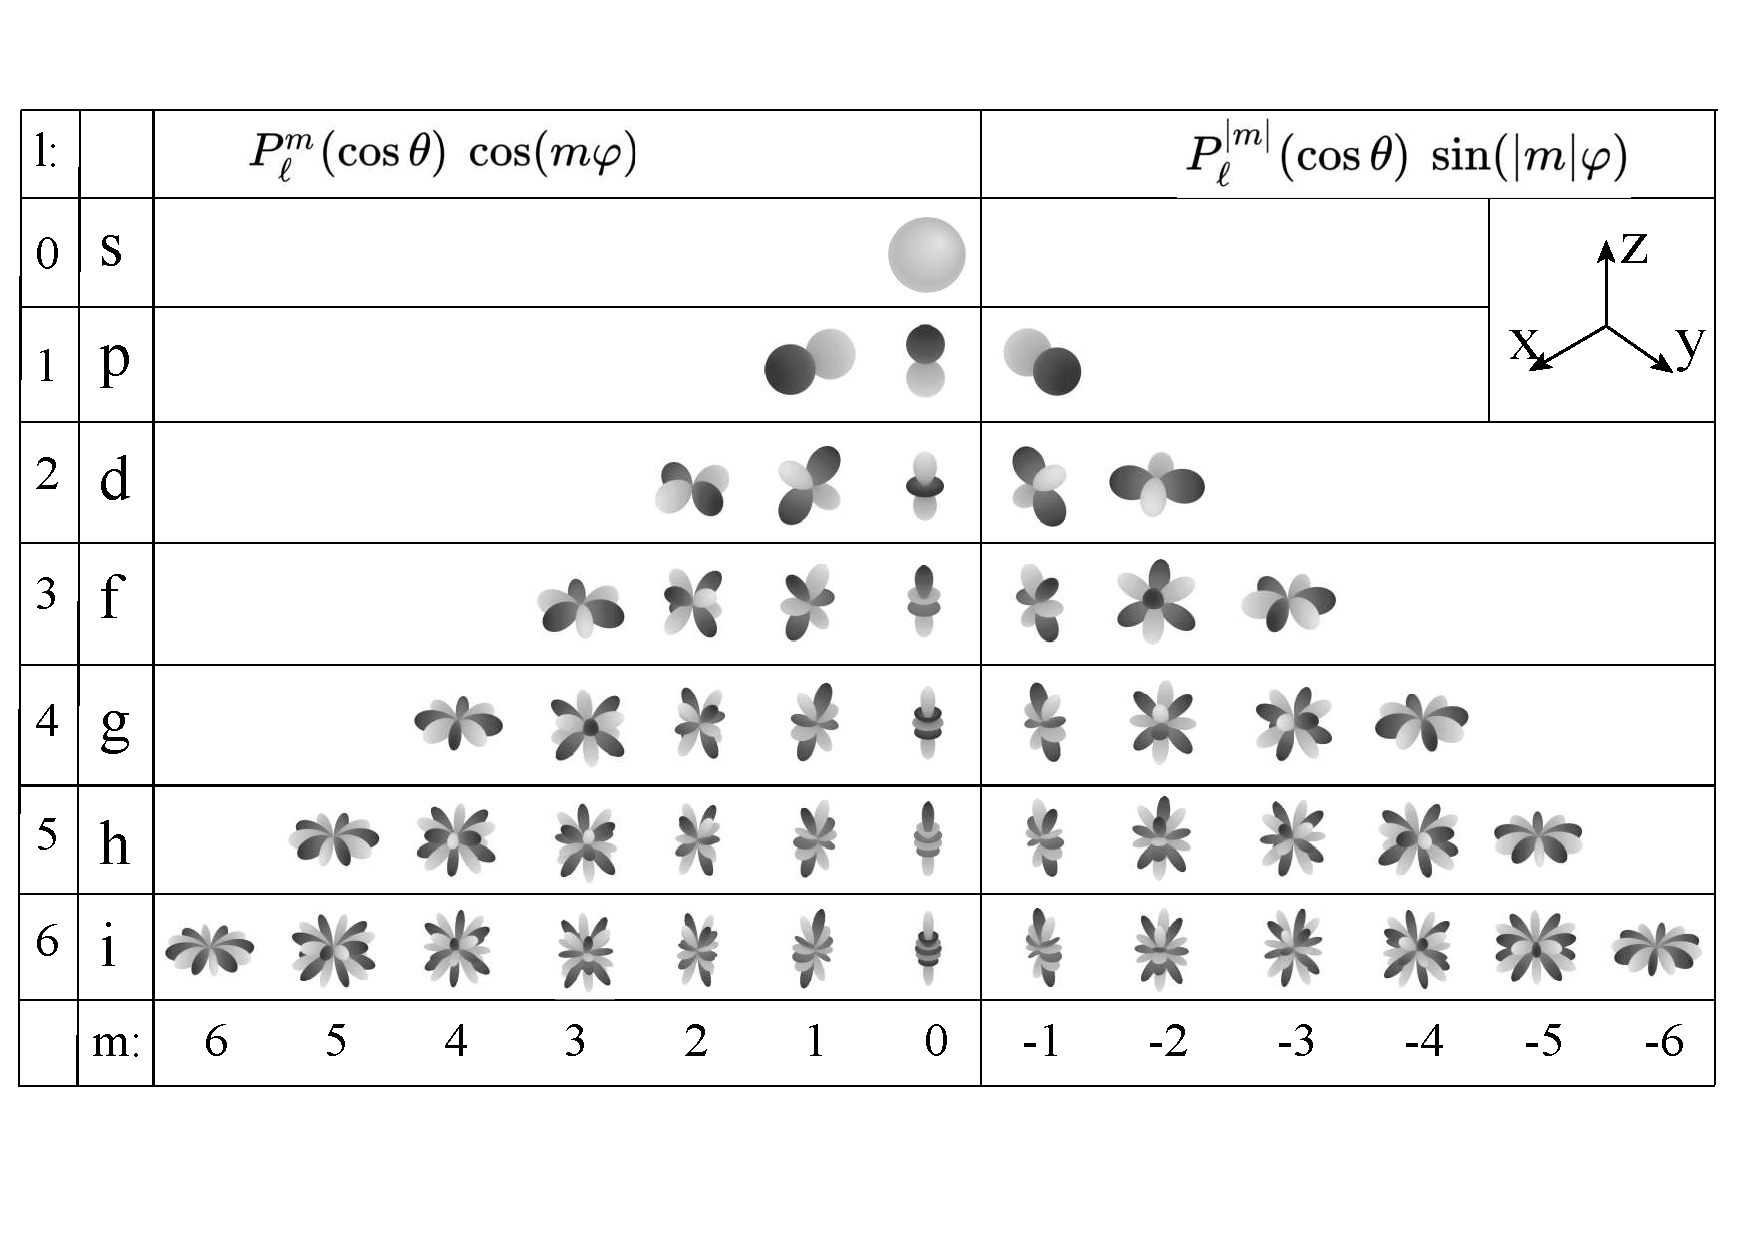
\includegraphics[page=1,width=\textwidth]{pictures/Sphericalfunctions.pdf}
	\caption{Reelle Spherical Harmonics. Der Abstand zum 0-Punkt korrespondiert zum Betrag von $Y_l^m$, die helle Oberfläche zeigt positive Werte von $Y_l^m$, dunkle Oberfläche negative Werte an.}
\end{figure}
